\documentclass{article}\usepackage{multirow}\usepackage{changepage}\usepackage{graphicx}\usepackage[fleqn]{amsmath}\usepackage{amssymb}\title{Young's Double Slit Lab}\author{Tristan, Ibrahim, Oliver, Aaliya}\begin{document}\maketitle\section*{Purpose}{The purpose of this lab was to measure the wave length ($\lambda$) of a laser travelling through a slit, then calculate the error percentage produced by our result.}\section*{Materials}\begin{itemize}\item {{\textbf{One} Slit}}\item {{\textbf{One} Line of Measuring Tape}}\item {{\textbf{One} Red Laser}}\item {{\textbf{One} Projector}}\item {{\textbf{Two} Rulers}}\item {{\textbf{One} Piece of Paper}}\end{itemize}\leavevmode\section*{Procedure}\begin{enumerate}\item {{The sheet of paper was taped to the black-board.}}\item {{The laser was positioned infront of the slit, both facing the piece of paper on the black-board.}}\item {{Using a pencil, the blocks made by the laser and slit were marked on the piece of paper.}}\item {{The distance between the middles of two blocks made by the laser and slit was measured. ($\Delta x$)}}\item {{The distance from the slit to the black-board was measured. ($L$)}}\item {{The width of the slits' double-line was measured using the projector, two rulers, and the slit itself. ($d$)}}\end{enumerate}\leavevmode\section*{Observations}{During our experiment, our group made the following observations. Below exhibits the distance from the slit to the black-board ($L$) and the distance from the middles of two blocks projected by the laser travelling through our slit. ($\Delta x$)}\begin{itemize}\item {{$L$ $\approx$ $73cm$ $\approx$ $7.3m$}}\item {{$\Delta x$ $\approx$ $0.7cm$ $\approx$ $7.0\times 10^{-3}$ $m$}}\end{itemize}\leavevmode\section*{Caclulations: Solve for $d$}{Before solving for $\lambda$, we must find $d$ (the width of the slit). To do this we used a projector (magnifier) and the formula below.\newline\newline}\begin{equation*}\therefore\;d\;=\;\frac{(1mm)(slit\;width\;on\;projection)}{(1mm\;on\;projection)}\;=\;\frac{(1mm)(3.2mm)}{(6.1mm)}\;\approx\;5.24\times\;10^{-4}m\end{equation*}\newline\section*{Calculations: Solve for $\lambda$}{After finding $d$ we can solve for $\lambda$ by substituting our previous variables into the following equation.\newline\newline}\begin{equation*}\therefore\;\lambda\;=\;\frac{\Delta\;xd}{L}\;=\;\frac{(7.0\times\;10^{-3})(5.24\times\;10^{-4})}{(7.3)}\;\approx\;5.02\;\times\;10^{-7}m\end{equation*}\newline\section*{Calculations: Error Percentage}{After solving for our experimental result, we use the error percentage formula to find how accurate our results really were.}\begin{equation*}\therefore\;Error\;\%\;=\;\left(\frac{Experimental\;-\;Theoretical}{Theoretical}\right)\;\times\;100\end{equation*}\begin{equation*}\therefore\;Error\;\%\;=\;\left(\frac{(5.02\;\times\;10^{-7})\;-\;(6.53\;\times\;10^{-9})}{(6.53\;\times\;10^{-9})}\right)\;\times\;100\;\approx\;>\;100\;\%\end{equation*}\section*{Sources of Errors}\begin{enumerate}\item {{The blocks projected by the laser travelling through the slit were too close together. This made measuring the distances far harder and far more inaccurate.}}\item {{Measuring from the projector made achieving accurate results far more difficult due to how large and pixelated the projection is.}}\item {{The laser was too far away / too close to the the slit.}}\end{enumerate}\leavevmode\section*{Solutions to Errors}\begin{enumerate}\item {{Move to a larger space so we can station the materials accordingly.}}\item {{Use a higher resolution projector or have each of our group members measure values then calculate the average of the results.}}\item {{Measure an appropriate distance for the laser away from the slit.}}\end{enumerate}\leavevmode\section*{Conclusion}{Therefore, upon the conclusion of this lab it was determined that the wave length ($\lambda$) of a laser travelling through a slit was approximately $5.02\;\times 10^{-6}m$ though because of the experimental errors documented above, this result produced a high error percentage of approximately $7.6\times 10^5\;\%$}\section*{Pictures}{The image below is the result of the laser travelling through our provided slit. The blocks being projected by the laser and slit were very close together and fuzzy. This was one of the prime sources of errors that was documented above.\newline\newline}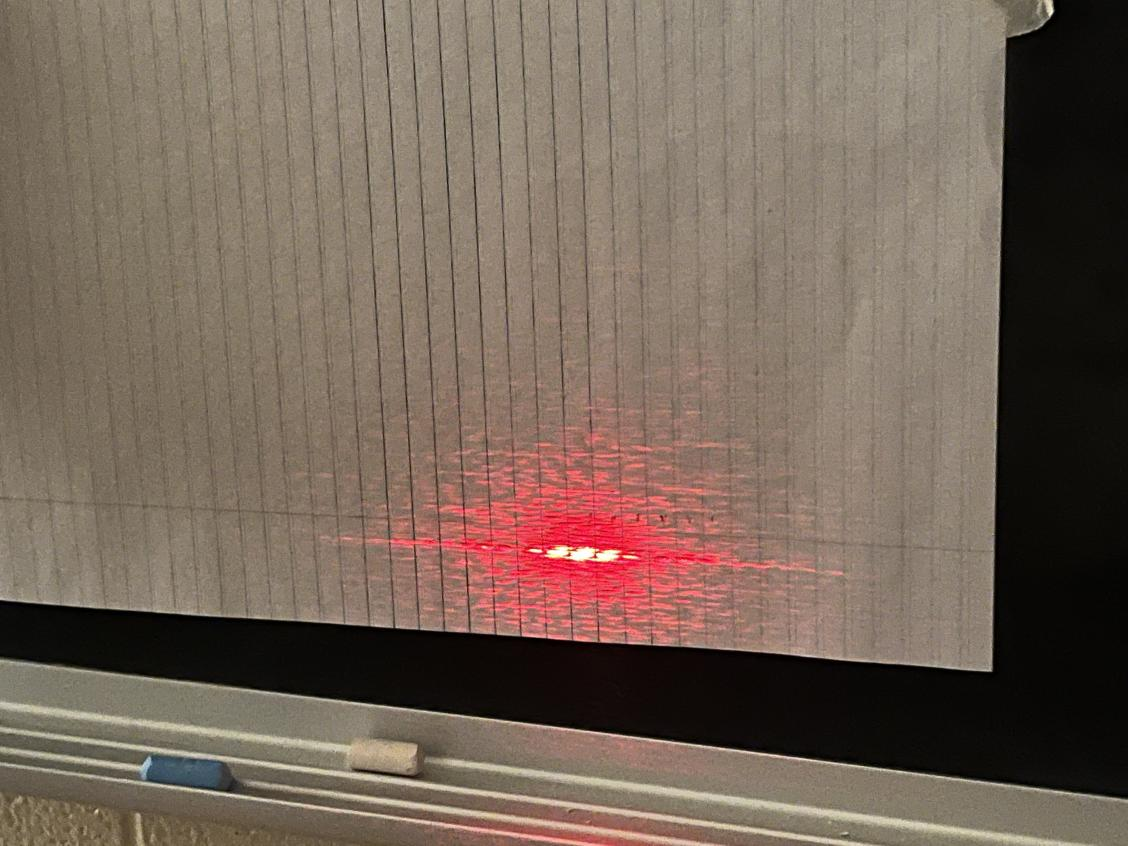
\includegraphics[scale=0.15]{/Users/tristan/Desktop/LaTeX/Physics Light + Waves/Young's Double Slit Lab//images/laser_split.png}\end{document}